\subsection{Verwendete Tools (DH)}
Die nachfolgenden Abschnitte erläutern die eingesetzten Werkzeuge, die für das Projekt benötigt werden.

\subsubsection{Tools zur Erstellung von Videos (DH)}
Um dem Kunden den aktuellen Stand der Entwicklung zu präsentieren, werden Videos von den Teilfunktionen der Software angefertigt. Anhand dieser Videos kann der Kunde Feedback zur Software geben, ohne jedes mal eine neue Version der Software installieren zu müssen. Darüber hinaus dienen die Videos später auch dazu, die Software in Internet anzupreisen beziehungsweise Kunden einen Einblick in die Software zu gewähren. Außerdem werden die Videos der Software als Hilfe hinzugefügt.\\
Zur Erstellung von Videos werden zwei Werkzeuge benötigt: Das Open Broadcaster Studio und OpenShot. Diese beiden Tools können auf den Betriebssystemen Windows, MacOS und Linux verwendet werden und besitzen eine GPL-Lizenz. Die erstellten Videos dürfen folglich kommerziell benutzt werden.\bigskip \\
\textbf{Open Broadcaster Studio (DH)}\\
Mit dem Open Broadcaster Studio\footnote{https://obsproject.com/download} werden die Videos samt Ton aufgenommen. Die Anwendung ist in Abbildung \ref{fig:OBS} dargestellt.
\begin{figure}[htb]
	\centering
		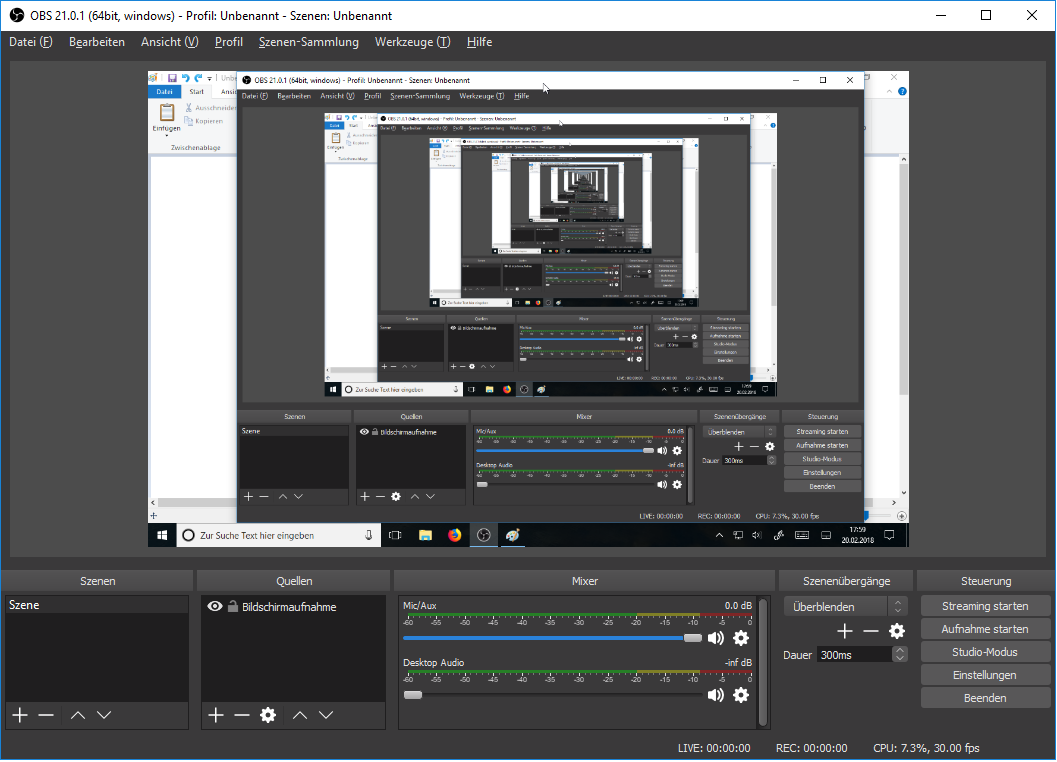
\includegraphics[width=0.70\textwidth]{figures/OBS.png}
	\caption{Open Broadcast Studio}
	\label{fig:OBS}
\end{figure}
Der Vorteil dieser Software ist, dass sie, anders als beispielsweise der VLC Media Player, die Video- und Audiosignale gleichzeitig aufnehmen kann \cite[vgl.][]{OBS}.\\
Nach der Installation führt die Anwendung eine automatische Konfiguration durch, dabei sollte die Konfiguration für die Aufnahme selektiert werden. Nach dieser Konfiguration kann überprüft werden, ob das Mikrofon gefunden wurde, indem die Signalstärke des Audiogeräts betrachtet wird. Sollte sich diese nicht beim Sprechen bewegen, so kann die Wahl des Audiogerätes über die Einstellungen vorgenommen werden. Per default wird kein Videosignal aufgenommen. Um eine Videoquelle hinzuzufügen, wird in der Quelle die Bildschirmaufnahme (mit +) ausgewählt. Um nicht ständig das erzeugte Video in ein mp4-Format zu konvertieren, ist es ratsam, unter Einstellungen - Ausgabe das Aufnahmeformat auf mp4 zu stellen. Das mp4-Format wird zwingend für Websiten benötigt, deshalb müssen Videos immer das mp4-Format haben! Eine Aufnahme wird mittels Aufnahme starten begonnen und mit Aufnahme beenden gestoppt. Die Aufnahmen befinden sich anschließend in der Regel unter "`Dieser PC"' - Videos. Dies kann über Datei - Zeige Aufnahmen herausgefunden werden \cite[vgl.][]{OBS}. \bigskip \\
\textbf{OpenShot (DH)}\\
Das Open Broadcast Studio hat einen Nachteil: Mit ihm können die aufgenommenen Videos nicht geschnitten werden. Das Programm OpenShot\footnote{https://www.openshot.org/download/} kann Videos im mp4-Format schneiden. Leider hat dieses Programm jedoch den Nachteil, dass es gerne einfriert oder abstürzt. Für die im Projekt notwendigen Schnitte kann dies jedoch akzeptiert werden. Die Anwendung ist in Abbildung \ref{fig:OpenShot} dargestellt.
\begin{figure}[htb]
	\centering
		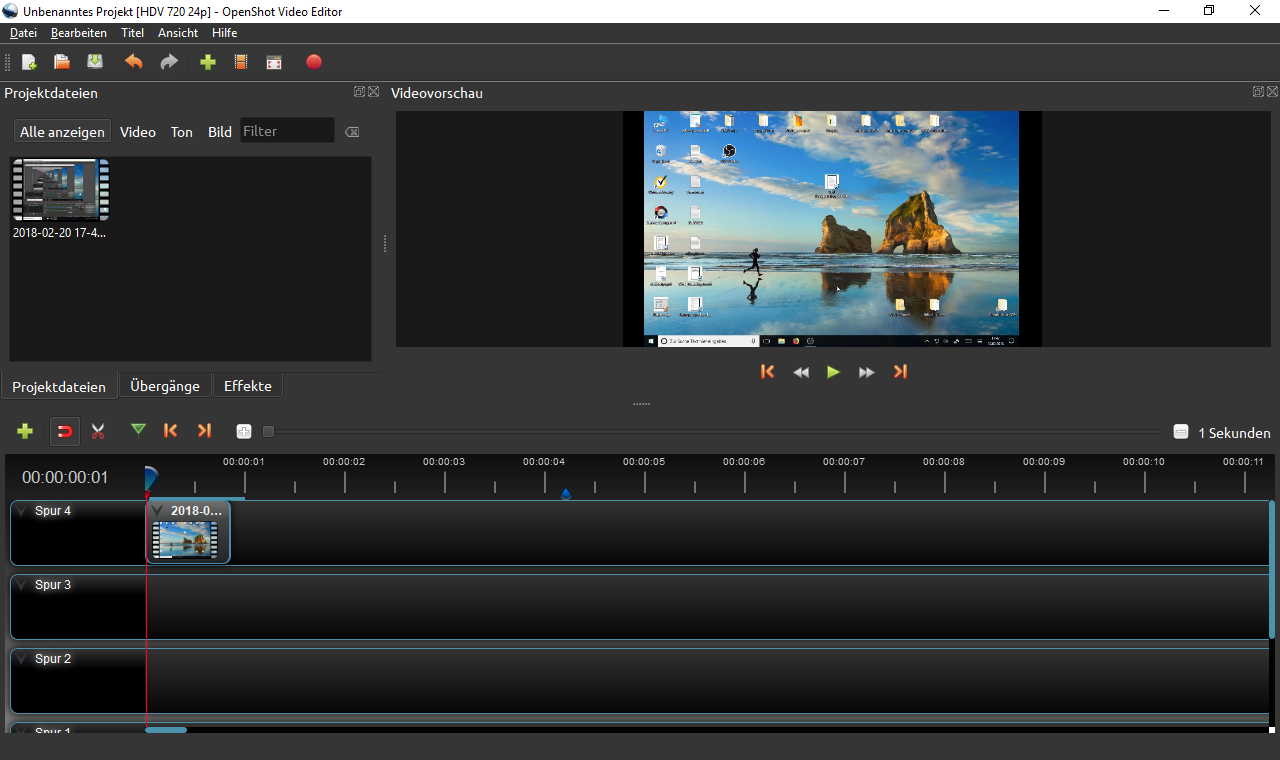
\includegraphics[width=0.70\textwidth]{figures/OpenShot.png}
	\caption{OpenShot}
	\label{fig:OpenShot}
\end{figure}
Um ein Video zu schneiden, wird im Feld Projektdateien per Rechtsklick Dateien importieren ausgewählt und die Datei selektiert, die geschnitten werden soll. Anschließend wird das importierte Video in eine Spur gezogen. Dabei sollte darauf geachtet werden, dass die Datei zum Zeitpunkt Null in der Spur liegt. Mit der roten Zeitachse wird die Stelle im Video gesucht, an der geschnitten werden soll. Ist die Stelle gefunden, wird das Schneidewerkzeug (Schere) selektiert und auf die markierte Stelle angewendet (Achtung: Dies kann etwas dauern!). Das Video wird an der entsprechenden Stelle aufgeteilt. Das Schneidewerkzeug muss nun deselektiert werden, um den Teil des Videos löschen zu können. Zum Löschen wird auf den gewünschten Teil mit Rechtsklick Video löschen ausgewählt (den Rest wieder an den Null-Punkt ziehen). Aus den Videos sollten alle Teile herausgeschnitten werden, die nicht unbedingt darin enthalten sein sollten. Dies ist zum Beispiel der Anfang und das Ende des Videos, in dem die Aufnahmefunktion gestartet beziehungsweise gestoppt wird. Zum Speichern des geschnitten Videos wird Datei - Video exportieren ausgewählt. Wichtig beim Speichern: Das Format muss erneut mp4 sein!

\subsubsection{TaskBoard (DH)}
Die einzelnen Aufgaben werden in einem TaskBoard, siehe Abbildung \ref{fig:TaskBoard}, festgehalten und können agil bearbeitet werden. Jeder Teilnehmer des Projektes erhält einen eigenen Account auf dem TaskBoard. Es kann unter https://gitlab-testbot.informatik.hs-augsburg.de/taskboard erreicht werden.
\begin{figure}[htb]
	\centering
		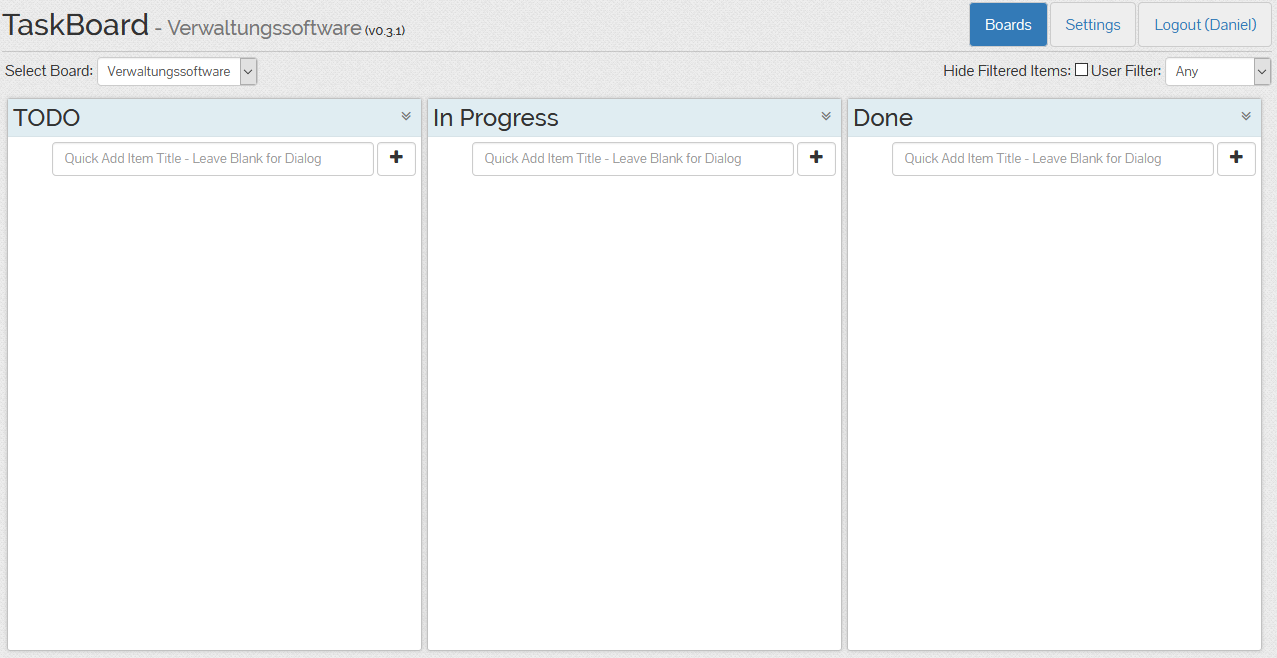
\includegraphics[width=0.70\textwidth]{figures/TaskBoard.PNG}
	\caption{TaskBoard}
	\label{fig:TaskBoard}
\end{figure}
Jedes Board des TaskBoards besteht aus drei Tabellen: 
\begin{itemize}
	\item TODO: Enthält Aufgaben, die noch zu erledigen sind
	\item In Progress: Aufgaben, die von einer Person derzeit bearbeitet werden
	\item Done: Erledigte Aufgaben
\end{itemize}
Die Einrichtung des TaskBoards ist in Anhang \ref{Anhang_TaskBoard} erläutert.\\
Jeder Eintrag des TaskBoards besteht aus den Informationen:
\begin{itemize}
	\item Titel: Name des Eintrags im TaskBoard.
	\item Abhängig von: Aufgaben, die vor diesem Task erledigt sein müssen, da deren Ergebnisse für den Task benötigt werden.
	\item Voraussetzung für: Aufgaben, die die Ergebnisse dieses Tasks benötigen.
	\item Dauer: Geplante Zeit, die für die Erledigung der Aufgabe geschätzt wurde.
	\item Beschreibung: Detailierte Informationen zur Aufgabe.
\end{itemize}

\subsubsection{Entwicklungsumgebung (DH)}
Als Entwicklungsumgebung wird der QtCreator zusammen mit der Qt-Bibliothek\footnote{https://github.com/qt/qt5} verwendet. Qt 5.11 stellt bereits erste Funktionalitäten für die Sprachsteuerung bereit: Die Ausgabe von Sprache mit QTextToSpeech. Eine Spracheingabe besitzt Qt noch nicht, deshalb wird auf Voce\footnote{http://voce.sourceforge.net/} zurückgegriffen.

